\subsection{Proration Analysis and Decision}

Given the substantial data loss from excluding mid-year QSI changes, we investigated whether costs could be prorated for partial-year records. The analysis examined monthly cost distributions for all customers, calculating two metrics:

\begin{align}
q &= \frac{\text{months with services}}{12} \\
r &= \sum_{i=1}^{12} \frac{(m_i - \bar{m})^2}{\bar{m}}
\end{align}

where $m_i$ represents monthly expenses and $\bar{m}$ is the average monthly expense for that customer-year.

\begin{figure}[h]
    \centering
    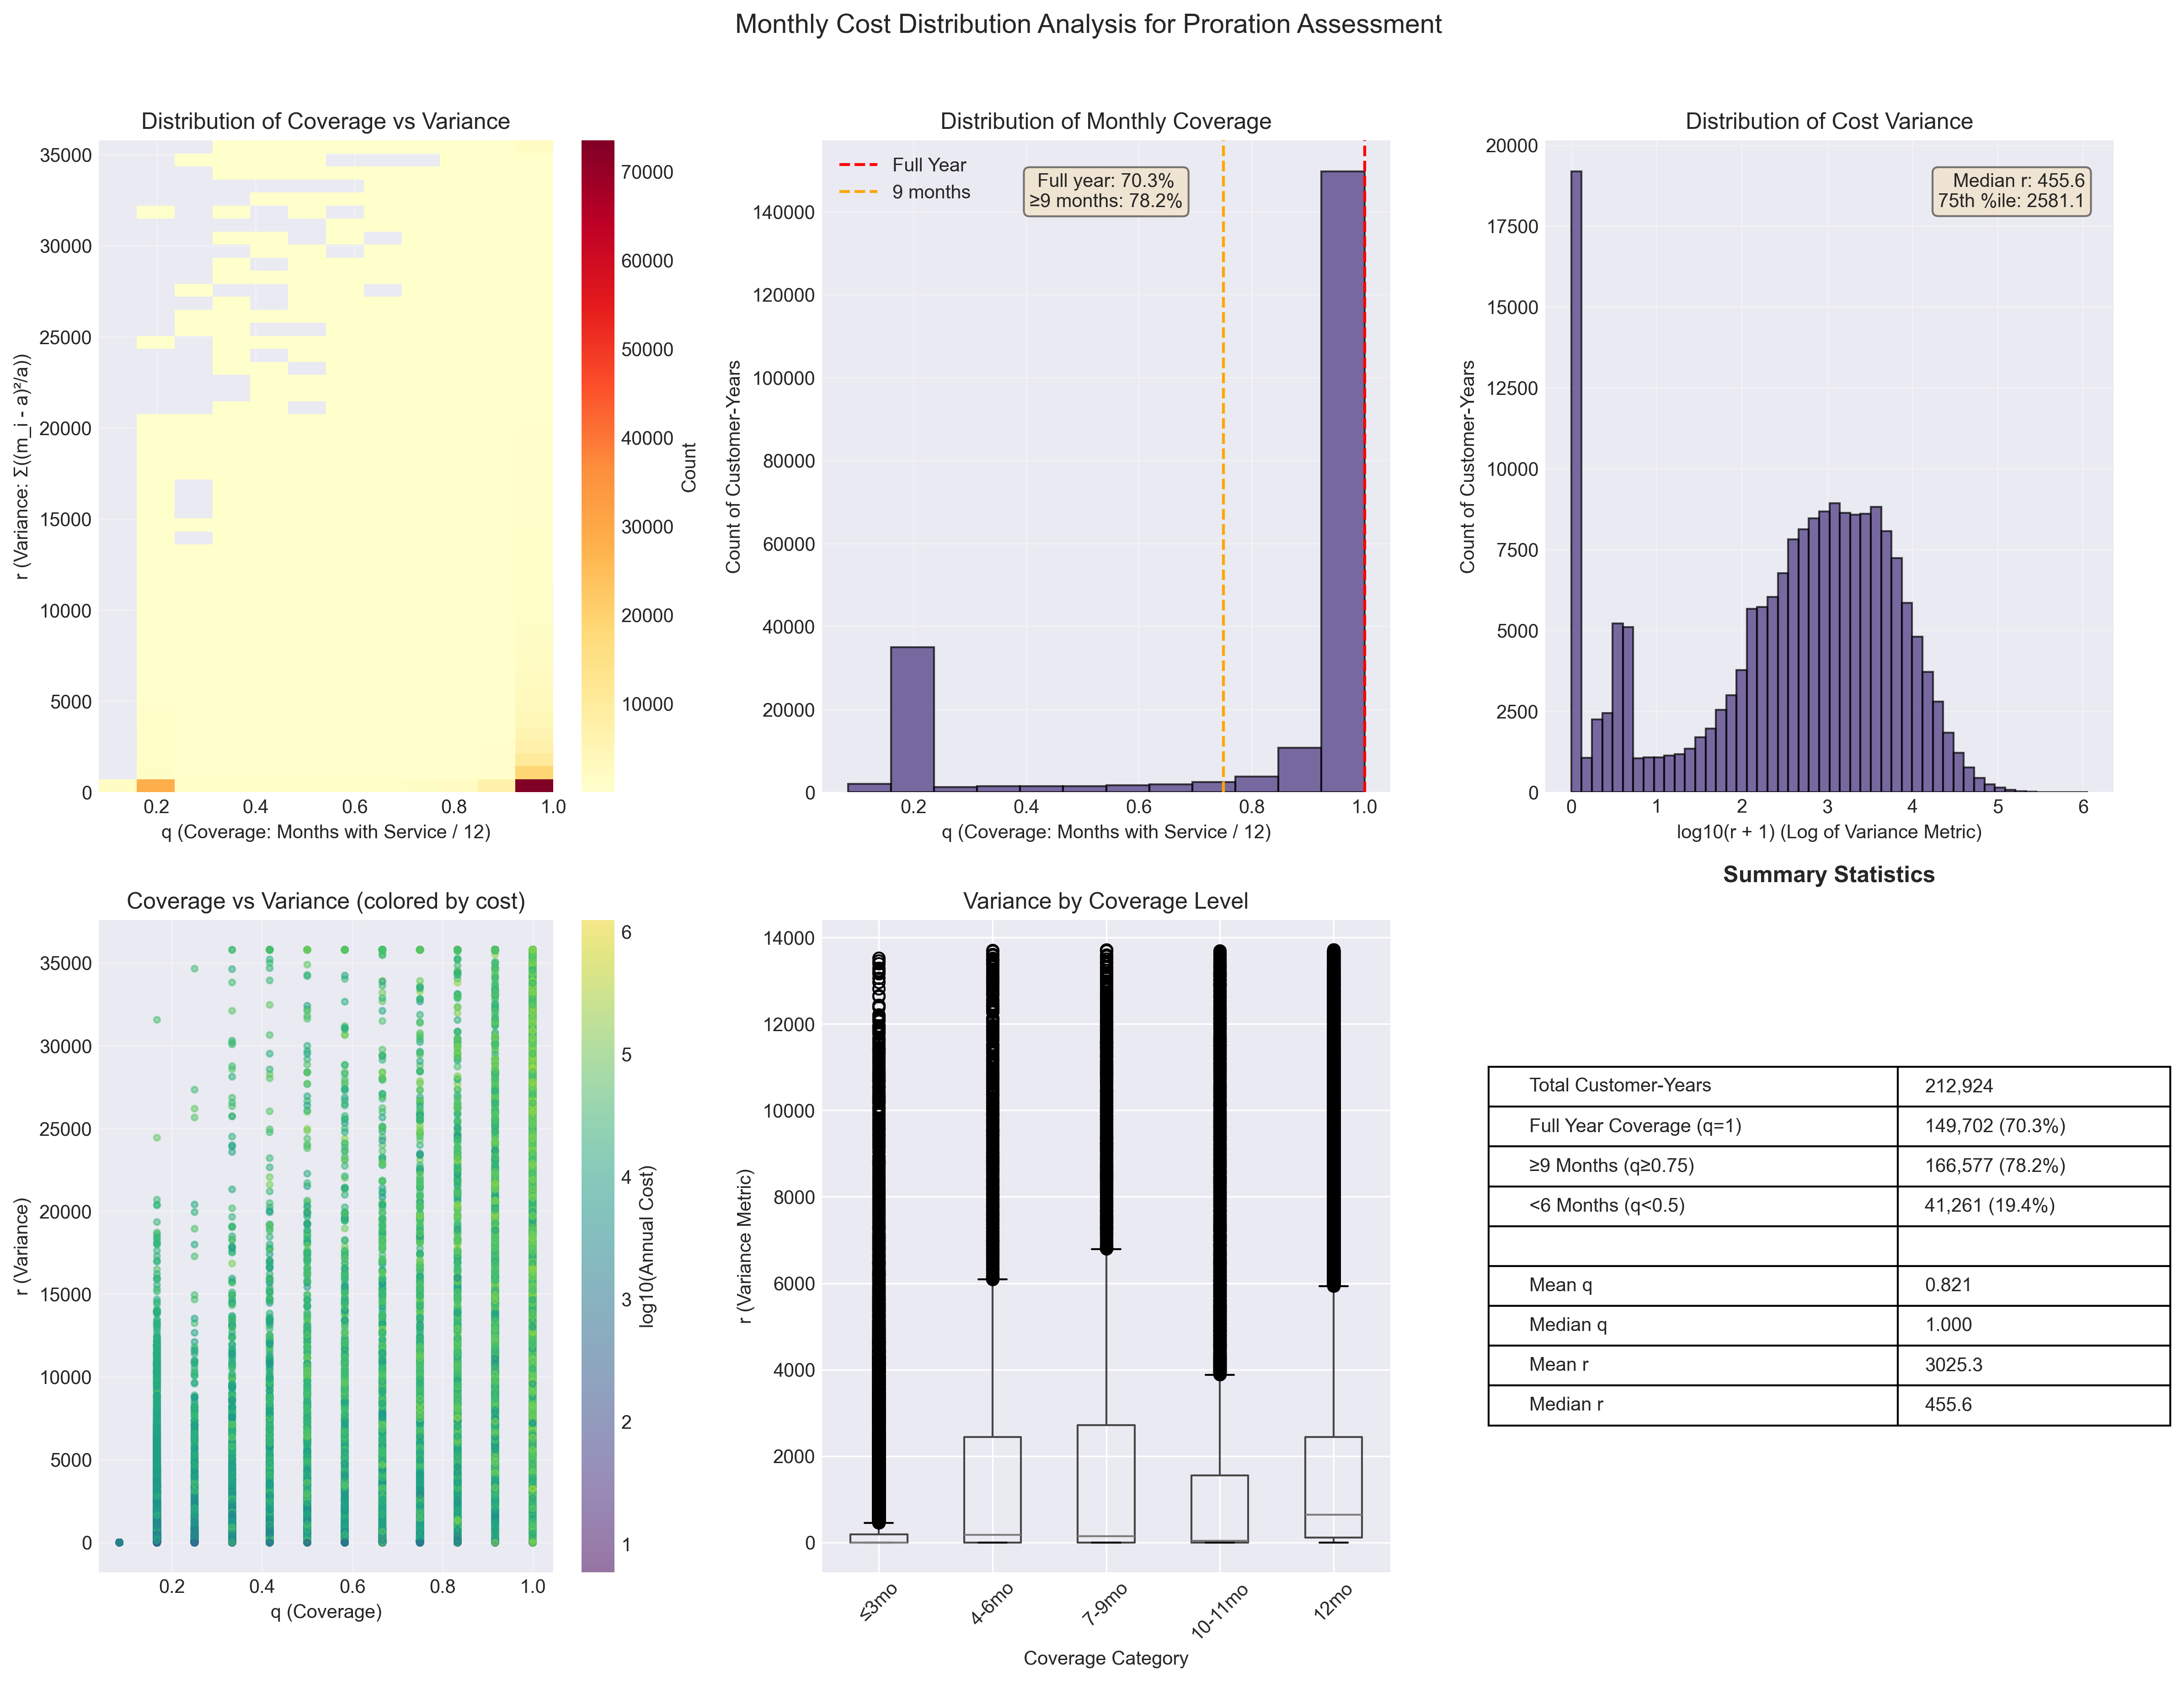
\includegraphics[width=\textwidth]{figures/cost_distribution_analysis.png}
    \caption{Monthly cost distribution analysis for proration assessment}
    \label{fig:proration_analysis}
\end{figure}

Figure~\ref{fig:proration_analysis} presents the comprehensive proration feasibility analysis:

\begin{itemize}
    \item \textbf{Top-left panel}: Two-dimensional histogram showing the relationship between coverage ($q$) and variance ($r$). The concentration of points at $q=1$ demonstrates that most customer-years have complete coverage, while the vertical spread indicates substantial variance in spending patterns.
    
    \item \textbf{Top-center panel}: Distribution of monthly coverage showing a bimodal pattern---customers either have full-year coverage or very limited engagement, with few in between.
    
    \item \textbf{Top-right panel}: Log-scale distribution of the variance metric revealing that cost variance spans multiple orders of magnitude, indicating highly heterogeneous spending patterns.
    
    \item \textbf{Bottom-left panel}: Scatter plot colored by annual cost magnitude shows that higher-cost customers tend to have more complete coverage but also higher variance.
    
    \item \textbf{Bottom-center panel}: Box plots of variance by coverage category reveal the counterintuitive finding that full-year customers have the highest cost variance.
    
    \item \textbf{Bottom-right panel}: Summary statistics quantifying the distribution patterns.
\end{itemize}

The analysis revealed critical findings:
\begin{itemize}
    \item \textbf{\ProrationFullYearPct\% of customer-years} have full 12-month coverage ($q = 1.0$)
    \item \textbf{Median variance for full-year customers}: $r = \ProrationMedianRFull$
    \item \textbf{Median variance for low-coverage customers}: $r = \ProrationMedianRLow$
\end{itemize}

The counterintuitively high variance (\ProrationMedianRFull) for full-year customers indicates highly irregular spending patterns---likely reflecting equipment purchases, hospitalizations, or seasonal service variations. This ``lumpy'' cost distribution makes proration inadvisable for several reasons:

\begin{enumerate}
    \item \textbf{Attribution ambiguity}: With such high monthly variance, costs cannot be fairly attributed to different QSI assessment periods when changes occur mid-year.
    
    \item \textbf{Systematic bias}: The inverse relationship between coverage and variance suggests partial-year customers represent a fundamentally different population that would bias model calibration.
    
    \item \textbf{Implementation complexity}: Any proration scheme would require sophisticated adjustment factors that vary by customer characteristics, introducing additional uncertainty.
\end{enumerate}

Consequently, we maintain the conservative exclusion strategy despite the data loss, as the integrity of the QSI-to-cost relationship is paramount for regulatory compliance and fair budget allocation.
